\documentclass[11pt]{article}

\usepackage{sbc-template}
\usepackage{graphicx,url}
\usepackage{multirow}
\usepackage[table,xcdraw]{xcolor}
\usepackage{lscape}
\usepackage{longtable}
\usepackage{pgfplots}
\usepackage[titletoc]{appendix}
\pgfplotsset{width=10cm,compat=1.9}
\usepgfplotslibrary{external}
\tikzexternalize
\usepackage[utf8]{inputenc}
%\usepackage[brazil]{babel}
\usepackage[latin1]{inputenc}  
\usepackage{pdfpages}
\usepackage{listings}
\usepackage{color}
\usepackage{pdflscape}

%New colors defined below
\definecolor{codegreen}{rgb}{0,0.6,0}
\definecolor{codegray}{rgb}{0.5,0.5,0.5}
\definecolor{codepurple}{rgb}{0.58,0,0.82}
\definecolor{backcolour}{rgb}{0.95,0.95,0.92}

%Code listing style named "mystyle"
\lstdefinestyle{mystyle}{
  backgroundcolor=\color{backcolour},   commentstyle=\color{codegreen},
  keywordstyle=\color{blue},
  numberstyle=\tiny\color{codegray},
  stringstyle=\color{codepurple},
  basicstyle=\footnotesize,
  breakatwhitespace=false,         
  breaklines=true,                 
  captionpos=b,                    
  keepspaces=true,                 
  numbers=left,                    
  numbersep=5pt,                  
  showspaces=false,                
  showstringspaces=false,
  showtabs=false,                  
  tabsize=2
}
\lstset{style=mystyle}
\sloppy

\title{Comparison of Path Planning Algorithms\\ }
\author{Karelia A. Vilca\inst{1}}

\address{Instituto de Ciências Matemáticas e de Computação -- Universidade de São Paulo
  (USP) \\ -- São Carlos, SP -- Brazil\\
  \email{\ karelia@usp.br}
}

\begin{document} 
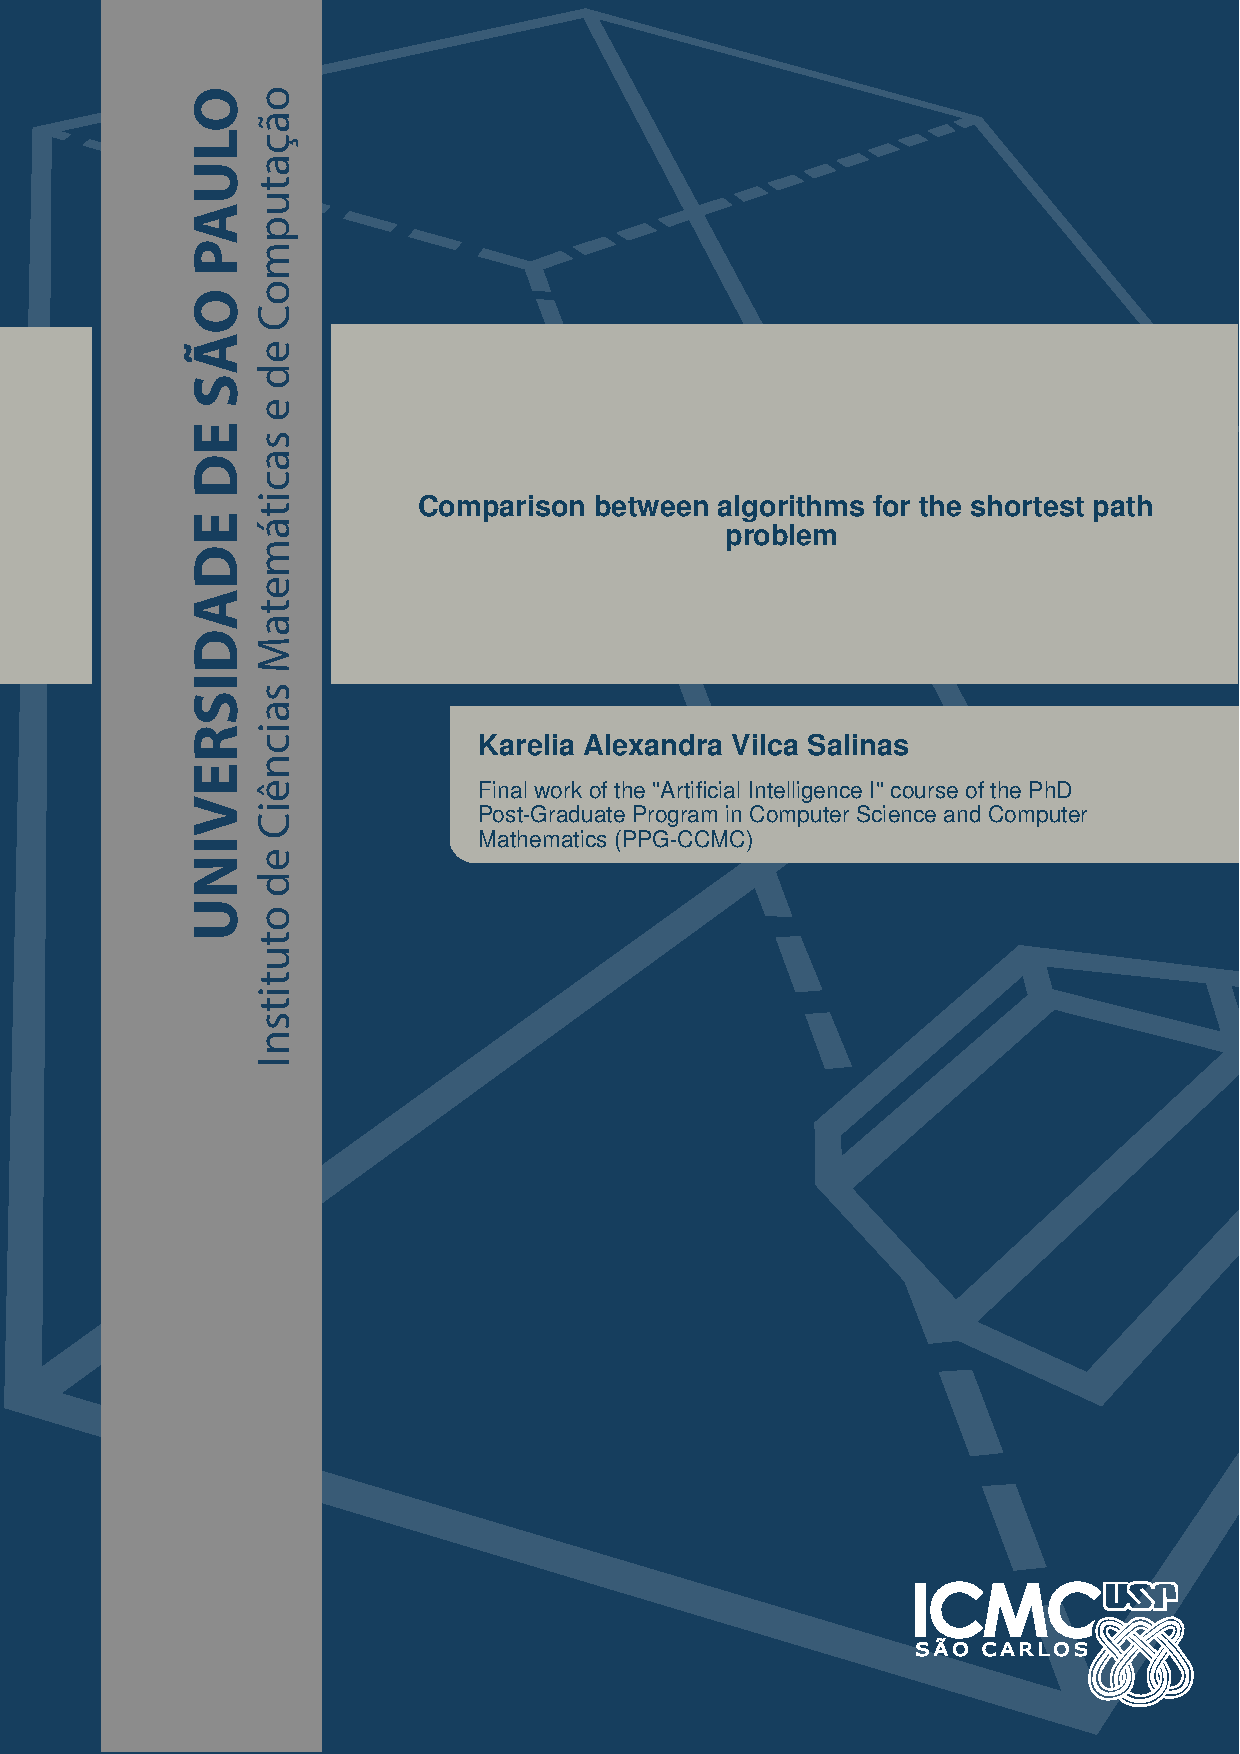
\includepdf{Template_SBC/file.pdf}

\maketitle

\begin{abstract}
This paper aims to compare the depth-first search, breadth-first search, A* and hill climbing algorithms applied to the path planning problem between two points. For this, all the methods were implemented and they were tested in random graphs with a different number of nodes, these graphs can be complete or not. The program allows to visualize the graph and to know the execution time, the cost and the length of the path, data that are contrasted with theoretical parameters to determine which one best suits the problem. 
\end{abstract}
\section{Introduction}
Road planning is a widely investigated problem, there are multiple investigations such as robotics \cite{shwail2013probabilistic}, route optimization, etc. Likewise, there are different solution algorithms proposed, including informed and non-informed searches, as well as proposals that mix methods such as \cite{felner2003kbfs}.

The objective of the present work is to compare the performance of 4 algorithms, depth-first search, breadth-first search, A* and hill climbing applied in the road planning problem between two points. The implementation allows indicating a number of nodes and choosing between constructing a complete graph or not and provides the routes taken and details of time, cost, etc.

In this work some of the typical problems such as "Shortest path problem" and "Travel Salesman Problem" are explained. Next, two blind search algorithms and two heuristic algorithms are developed with implementation details. And finally the results obtained are shown and compared.

\section{Path planning problems}
The routing problem is defined in terms of specified positions and transitions over links between them \cite{russell2004inteligencia}. 
To represent this type of problem, graphs or trees are used as data structures and the objective is achieved through search algorithms.
They can vary in the restriction of going through all the points or finding the direct route, as the well-known road problem from Arad to Bucharest \cite{russell2004inteligencia}, likewise some methods find any possible way and others try to optimize finding the least expensive solution. Some of the problems are listed below.

    \subsection{Shortest path problem}
    Let $G =  (V, E)$ be a graph with  vertex  set $V$ of size $n$ and arc set $E$ of size $m$. Let $s$ be a distinguished  vertex  of $G$ and let c be a function  assigning a non negative  real valued cost to each arc of $G$. We denote the cost by $c(v,w)$. The single-source shortest path problem is that  of computing, for each vertex  $v$ reachable from  $s$, the cost of a minimum-cost  path  from  $s$ to  $v$ \cite{ahuja1990faster}. 
    There are variations of this problem explained in \cite{dreyfus1969appraisal}; for example the shortest path problem between a specified pair of nodes or between all pair of nodes of a network. In 1959, Dijkstra \cite{dijkstra1959note} described the most efficient procedure for for this problem. 
    
    \subsection{Travel Salesman Problem}
    \cite{little1963algorithm} describe this problem as a salesman, starting in one city, wishes to visit each of $n-1$ other cities and return to the start. And the question is; in what order should he visit the cities to minimize the total distance traveled? Distance (time or cost) or costs between all city pairs are presumed known.
    It is closely related to the hamiltonian-cycle problem and that's why it's considered NP-complete \cite{cormen2009introduction}. Reference \cite{bellmore1968traveling} discusses methods of solution including Dynamic Programming.

\section{Search algorithms}
There are different algorithms for traversing or searching tree or graph data structures. For the search task, they can be grouped into blind search algorithms and algorithms of heuristic search.

    \subsection{Blind Search Algorithms (Uninformed)}
    According to \cite{russell2004inteligencia}, these strategies do not have additional information on states, as well as those provided by the definition of the problem. All search strategies are distinguished by the order in which we are expanded. An example shows DFS and BFS.

        \subsubsection{Depth-first search (DFS)}
        It was invented by Charles Pierre Trémaux (1859-1882) \cite{tremaux2010ecole} as a maze solving algorithm.
        This method implies, to search “deeper” in the graph whenever possible \cite{cormen2009introduction} and
        considers the following choice rule: when selecting an edge to traverse, always choose an edge emanating from the vertex most recently reached which still has unexplored edges \cite{tarjan1972depth}.
        It is neither complete nor optimal, but it has linear spatial complexity \cite{russell2004inteligencia}. In implementation terms it uses one LIFO (Last In, First Out) stack, it means that the most recently generated node is chosen for expansion \cite{russell2004inteligencia}.
        
        In the function \ref{DFS} is the implementation of the algorithm, it is considered a vector of booleans (\textit{visited}) to mark the nodes already visited and a stack (\textit{stack}). To start, the first node (\textit{coord\_ini}) is introduced to the stack. It then enters a loop that runs as long as the stack has elements to test or the target node (\textit{coord\_fin}) has not been found.
        In this loop the top node of the stack is extracted, this ensures the FIFO structure. It is verified if it has been visited. If it has not been visited yet, it is marked as visited and iterates through all its adjacencies adding them to the stack. The program will stop when it has found its target or in the worst case, when going through the whole tree it does not find the node indicated.
        \lstinputlisting[label=DFS,language=C++, caption=C ++ implementation of the DFS algorithm using a stack.]{codes/DFS.hpp}

        \subsubsection{Breadth-first search (BFS)}
        This method selects the shallow nodes for expansion; it is complete, great for unit cost steps, but it has exponential time complexity \cite{russell2004inteligencia}.
        While the depth search uses a LIFO, the breadth search uses a FIFO (First In, First Out) or queue. 
        
        For implementation \ref{BFS}, a queue is used to ensure FIFO behavior, it is started by doing push\_back of the start node. Then it goes into a loop that works as long as this queue has elements. Inside the loop, the node that has been in the queue for the longest time is obtained. If it has not been visited before, the visit is marked and its adjacencies are added to the queue. It also checks if the target node is between the adjacencies to stop the search.
        \lstinputlisting[label=BFS,language=C++, caption=Implementation of the BFS algorithm in C ++ using a queue.]{codes/BFS.hpp}

    \subsection{Heuristic Search Algorithms (Informed)}
    According to \cite{russell2004inteligencia}, an informed search strategy uses knowledge of a specific problem in addition to the definition of the problem itself and can find solutions more efficiently than a search strategy without information. In the case of path problem, they know if a non-objective state is “more promising” than another. It includes hill climbing, steepest hill climbing, A*, AO*, and Best First Search algorithms \cite{Maharshi2018ComparativeAO}.
        \subsubsection{A*}
        This method is the most widely know form of solution to the search for the best choice.
        It evaluates the nodes by combining:
        \begin{itemize}
            \item $g(n)$: the cost to reach the node. 
            \item $h(n)$: the cost to get from the node to the objective.
        \end{itemize}
        \begin{center}
            $f(n) = g(n) + h(n)$
        \end{center}
        So $f(n)$ is the estimated cost of the solution with the lowest cost through $n$.
        To find the lowest cost solution, it would be reasonable to try the node with the lowest value of $f(n)$ . As long as the heuristic function $h(n)$ satisfies certain conditions, the A * search will be complete and optimal. The algorithm is identical to the uniform cost search, except that A * uses $g + h$ instead of $g$ \cite{russell2004inteligencia}.
        
        For the implementation \ref{aa} of A*, the function 'a\_asterisk' receives a graph in the form of an adjacency matrix with the calculated distances between nodes.
        The variable 'origin' will initially be the starting node, but it will advance to the different nodes of the route. Then a loop is executed until the target node is found, in which it is checked if the node has been visited and the best successor node is obtained with the function 'near\_a'. 
        'near\_a' receives a node as a parameter and iterates through all its neighbors, calculates the distance (or the cost if the graph were weighted) of each neighbor to the target node (dist) this would be $h(n)$, in addition to the distance of the node parameter to its neighbor(grafo[origin][i]) that would be $g(n)$. Then it is checked if the sum of both is less than the local minimum to establish it as a new minimum. After traversing all the neighbors, the best neighbor is returned and the parameter node is marked as traversed.
        \lstinputlisting[label=aa,language=C++, caption= Implementation of the A * algorithm in C ++]{codes/Aasterisk.hpp}

        \subsubsection{Hill Climbing}
        It is a mathematical optimization technique which belongs to the family of local search. It is simply a repetitive loop that moves continuously towards increasing value, that is, up the slope. The algorithm ends when it reaches a “peak” where no neighbor has a higher value. The algorithm does not maintain a search tree and, therefore, the data structure of the current node only needs to record the state and value of its objective function \cite{russell2004inteligencia}. It is similar to optimizing a function, looking for the combination of parameter values that make the function assume the best value.
        
        It works as follows; search among the closest nodes the closest to the target, select it and go towards it. The radius of vision is now limited to the proximity of the current node. Repeat the process. 
        The implementation \ref{hc} follows the same structure as the A *. It has a different heuristic function, it considers as the best successor node the one with the smallest distance to the target node, that is, it does not take into account the distance from its predecessor, thus reducing its field of vision, it is verified that it is a local search algorithm.
        \lstinputlisting[label=hc,language=C++, caption=C ++ implementation of the hill climbing algorithm.]{codes/HillClimbing.hpp}

\section{Implementation pipeline}
This section gives some details of the program, which is written entirely in C ++ and is made up of; a main.cpp file added in the first appendix \ref{appendix:main} and 4 files containing the 4 methods, the code and explanation of them was already given in the previous section.

The program allows creating a complete or incomplete graph with a number of nodes indicated, this graph is used to test the 4 methods already explained and returns the path, the path length, the execution time and cost (distance). The distance considered is the Euclidean of the random points distributed in 2D space.
It is also accompanied by the display of the graph and it is possible to alternate between the paths with different letters. In the figure \ref{fig:exampleFig1} it is possible to see the program interface and the data it shows.

Below is the pipeline and also the reference to the code attached in appendix \ref{appendix:main}.
\begin{enumerate}
    \subsection{Input}
    \item The user is asked to enter the number of nodes for the construction of the graph. (main function line 277)
    \item It is possible to choose between the option of constructing a complete graph, with all the nodes interlaced with each other, or incomplete. (main function line 280)
    \item The menu is displayed to be able to change the graph of the path corresponding to each method. (main function lines 282:286)
    \subsection{Processing}
    \item For each node 2 random numbers are generated that will be the coordinates (x, y), they are stored. (main function lines 289:294)
    \item An initial node and random destination are established, among those already generated. (main function lines 295:298)
    \item The 'Build\_graph' function is called to construct the graph. First generate an empty matrix of $n*n$. Then an adjacency matrix is generated containing the node-to-node distance. If the graph is complete, all the nodes will be linked, but if it is incomplete, the criterion taken is as follows. A tolerated limit distance is established between nodes to create an edge, in case the nodes are very distant, their union is not considered. (main function line 300 and Buil\_graph function lines 25:49)
    \item The 'Build\_tree' function is called, which builds the tree aided by the information in the graph. For each node it verifies its adjacencies and it is saved in a node and adjacency vector correlation. To avoid cycles and that the tree is very big, the following is done; all nodes are traversed with a for but only the adjacencies are verified from the position occupied by that node onwards. This could cause adjacencies to be lost, but they are actually considered in previous iterations. In addition to ensuring operation, the initial node will be at position 0 so that there is a path to its successors, another resource may be to ensure that the initial node has a lower position than the final node.(main function line 301 and Buil\_tree function lines 51:63)
    \item The function 'Algorithms' is called, which executes each of the methods in the following order DFS, BFS, A * and Hill Climbing. Stores each of the paths get the data. 
    \subsection{Output}
    \item Program displays the complete path, the length, the execution time and the cost, which in this case is the accumulated distance, using the 'Path' function. (main function line 302 and Algorithms function lines 93:133)
    \item The cost of a path is the sum of the costs of its edges.\cite{ahuja1990faster}. To compute it, it iterates through the points traveled and the distance between them is calculated in an accumulated sum.  (Path function lines 75:94)
    \subsection{Visualization}
    \item The graph, its nodes and vertices are visually displayed. The initial node is highlighted with red and the target node is white, the path is also distinguished in orange. Since displaying all paths is confusing, you can toggle to display each with its initial letter (d, b, a, h). You can also zoom to better visualize large graphs.The OpenGL Utility Toolkit (GLUT) Programming Interface \cite{kilgard1996opengl} was used for this representation. (Different functions lines 135:272)
\end{enumerate}
The code is also available in the following Github repository \href{https://github.com/Kareliavs/-USP-IA-FinalWork}
\begin{figure}[ht]
\centering
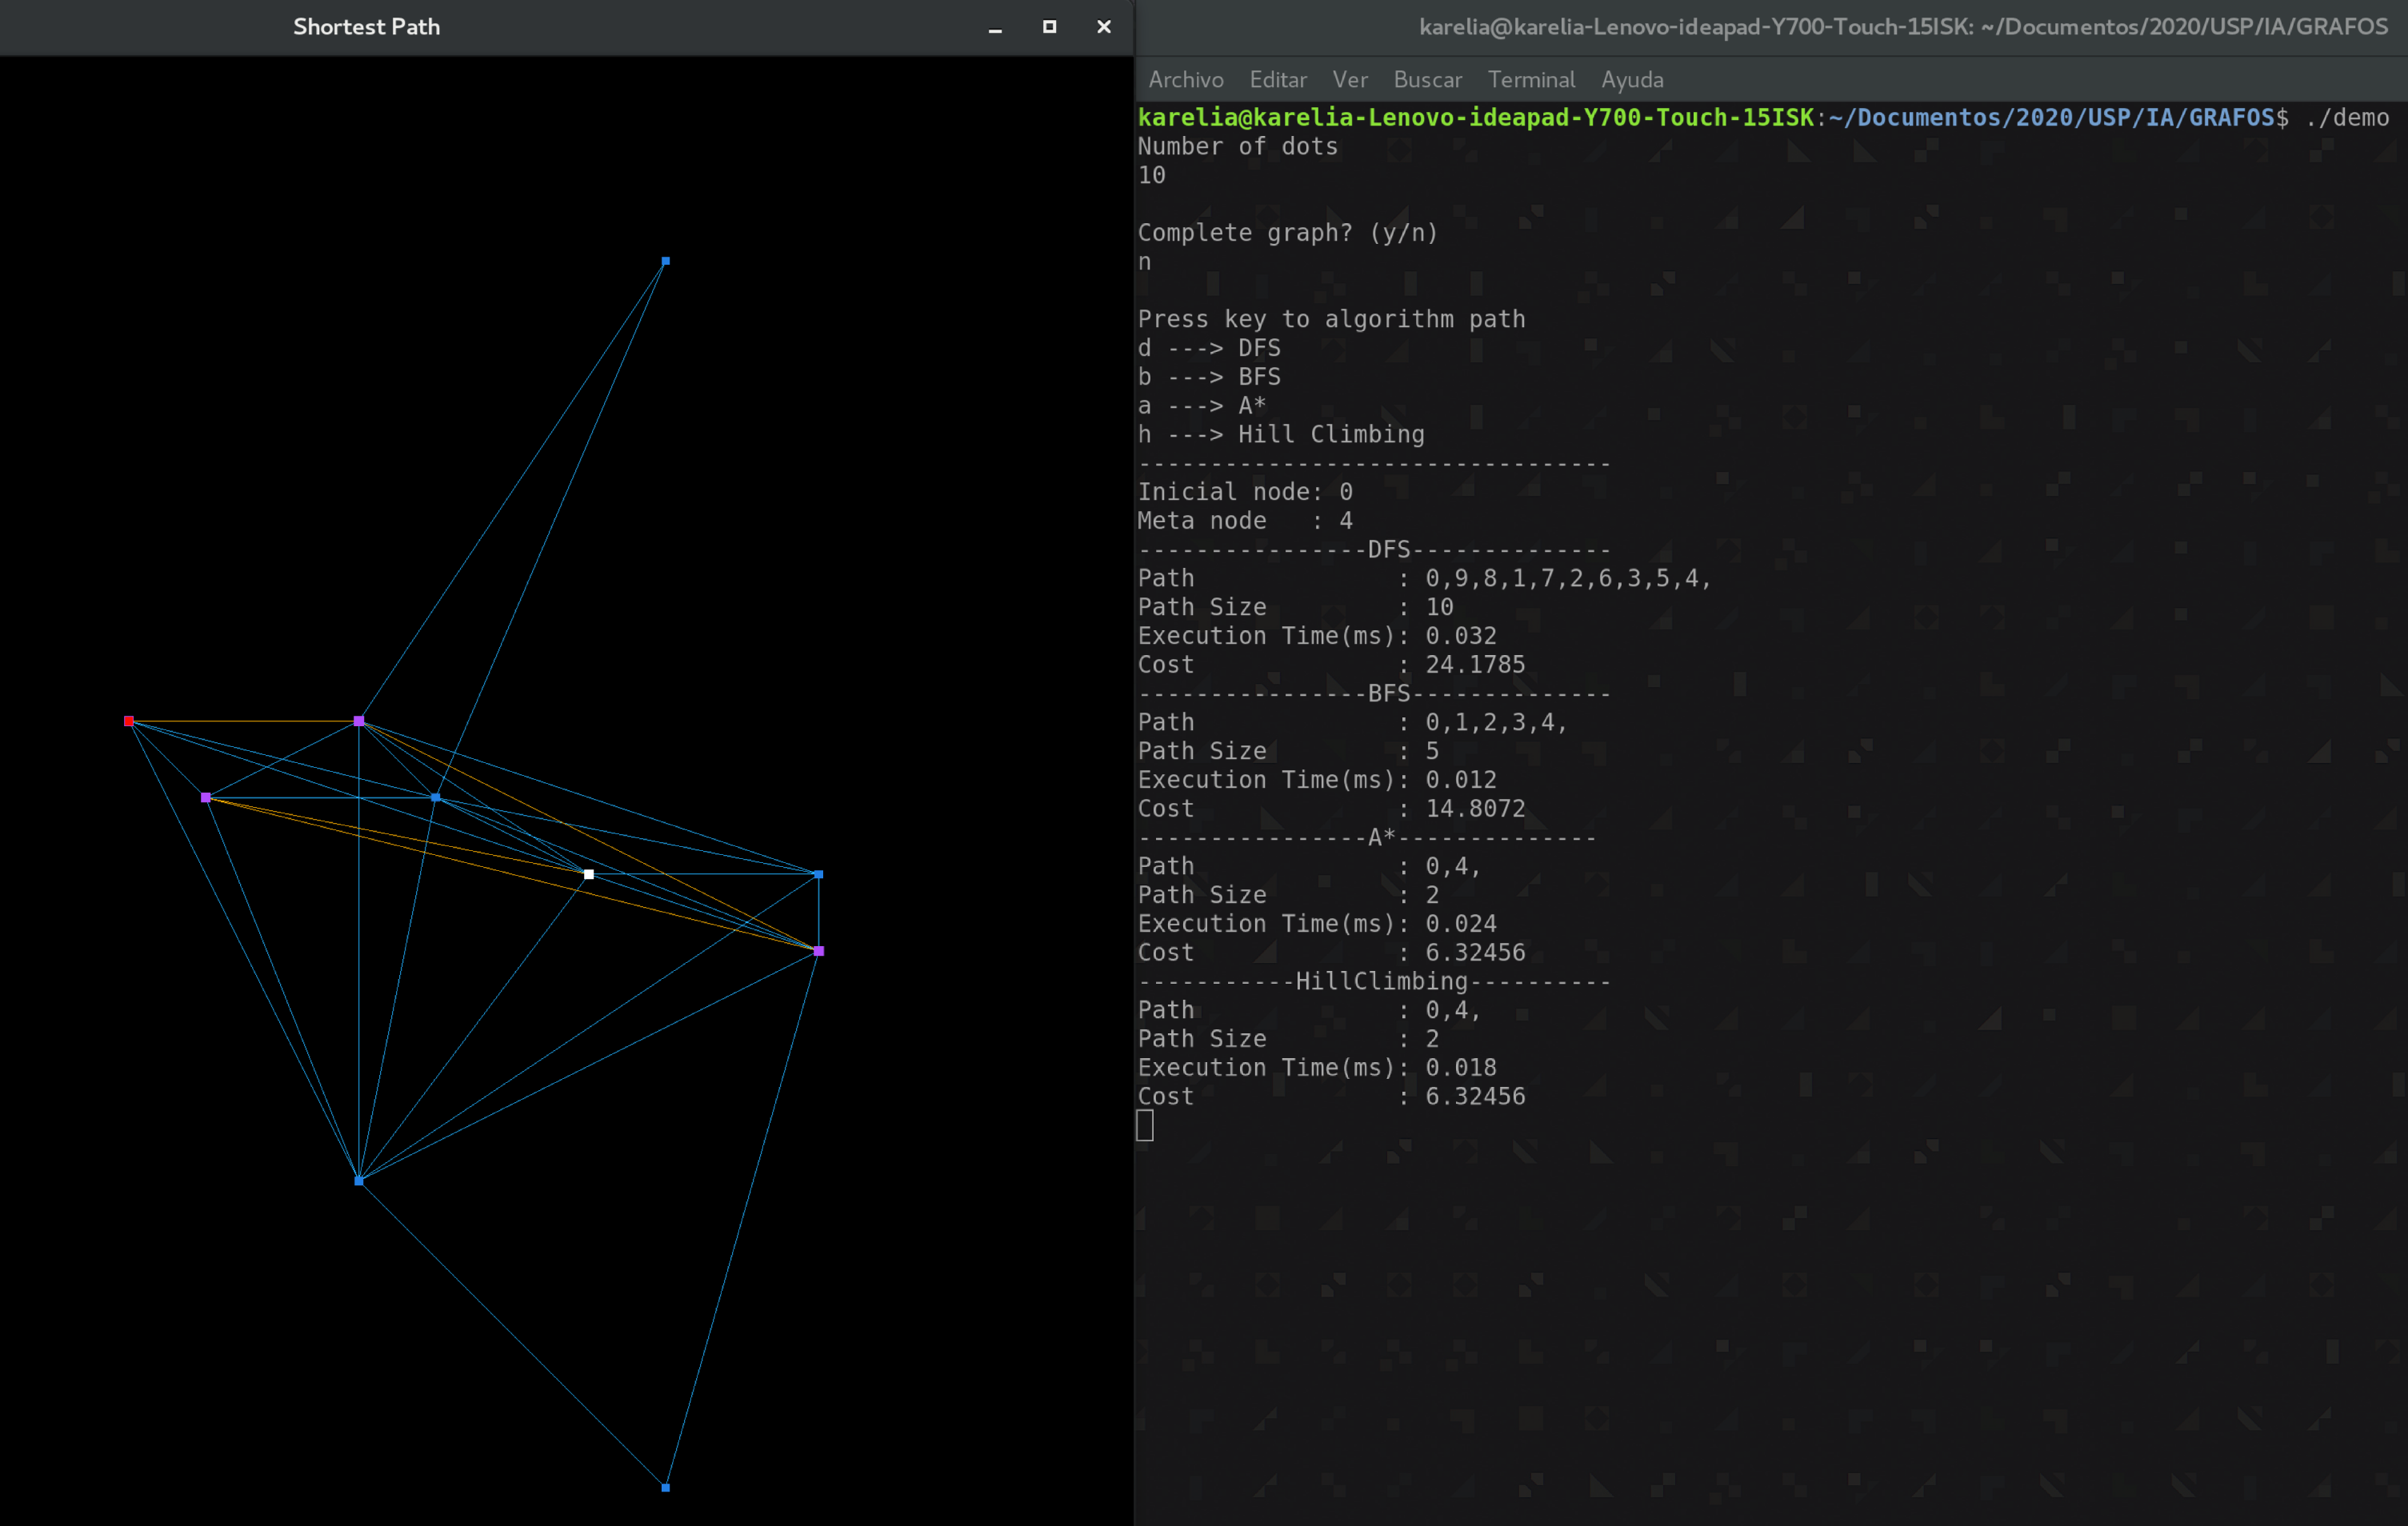
\includegraphics[width=0.8\textwidth]{Template_SBC/template-latex/screen.png}
\caption{The screenshot shows the development of the program. On the right side, the console shows how the number of nodes is entered by text, in this case 10, if it is a complete graph or not, in this case not and the initial node, meta node and the output of each of the methods, detailing the nodes traveled, the path length, the execution time in milliseconds and the cost or distance. On the right side the graph is shown as specified in the input, in blue the nodes and edges of the original graph are shown. The path shown in this example is a BFS that, as indicated in console, passes through 5 nodes highlighted in magenta, the path is drawn in orange and the starting node is highlighted in red and the target node in white. You can alternate the different paths by keyboard. For each of the examples, both graphic and textual output are shown.}
\label{fig:exampleFig1}
\end{figure}

\section{Experiments, results and comparison}
\subsection{Experiments}
In total 14 experiments were performed, for 7 different amounts of nodes (10, 50, 100, 500, 1000, 5000 and 10000) and for both complete and non-complete graphs. The program was restarted for each of the tests and the output data was recorded.

The figure \ref{fig:exampleFig2} shows the visualizations of 5 complete graphs of 10, 50, 100, 500 and 1000 nodes. It should be noted that when the graph is denser, the paths can hardly be perceived with the zoom tool, therefore they are not shown in this image.
The figure \ref{fig:exampleFig3} does the same for incomplete graphs of 10, 20, 50, 100 and 500 nodes. It can be seen that not all the nodes are linked, there is even the possibility that islands exist, this complicates the program but is also capable of detecting if there are no paths.

\begin{figure}[ht]
\centering
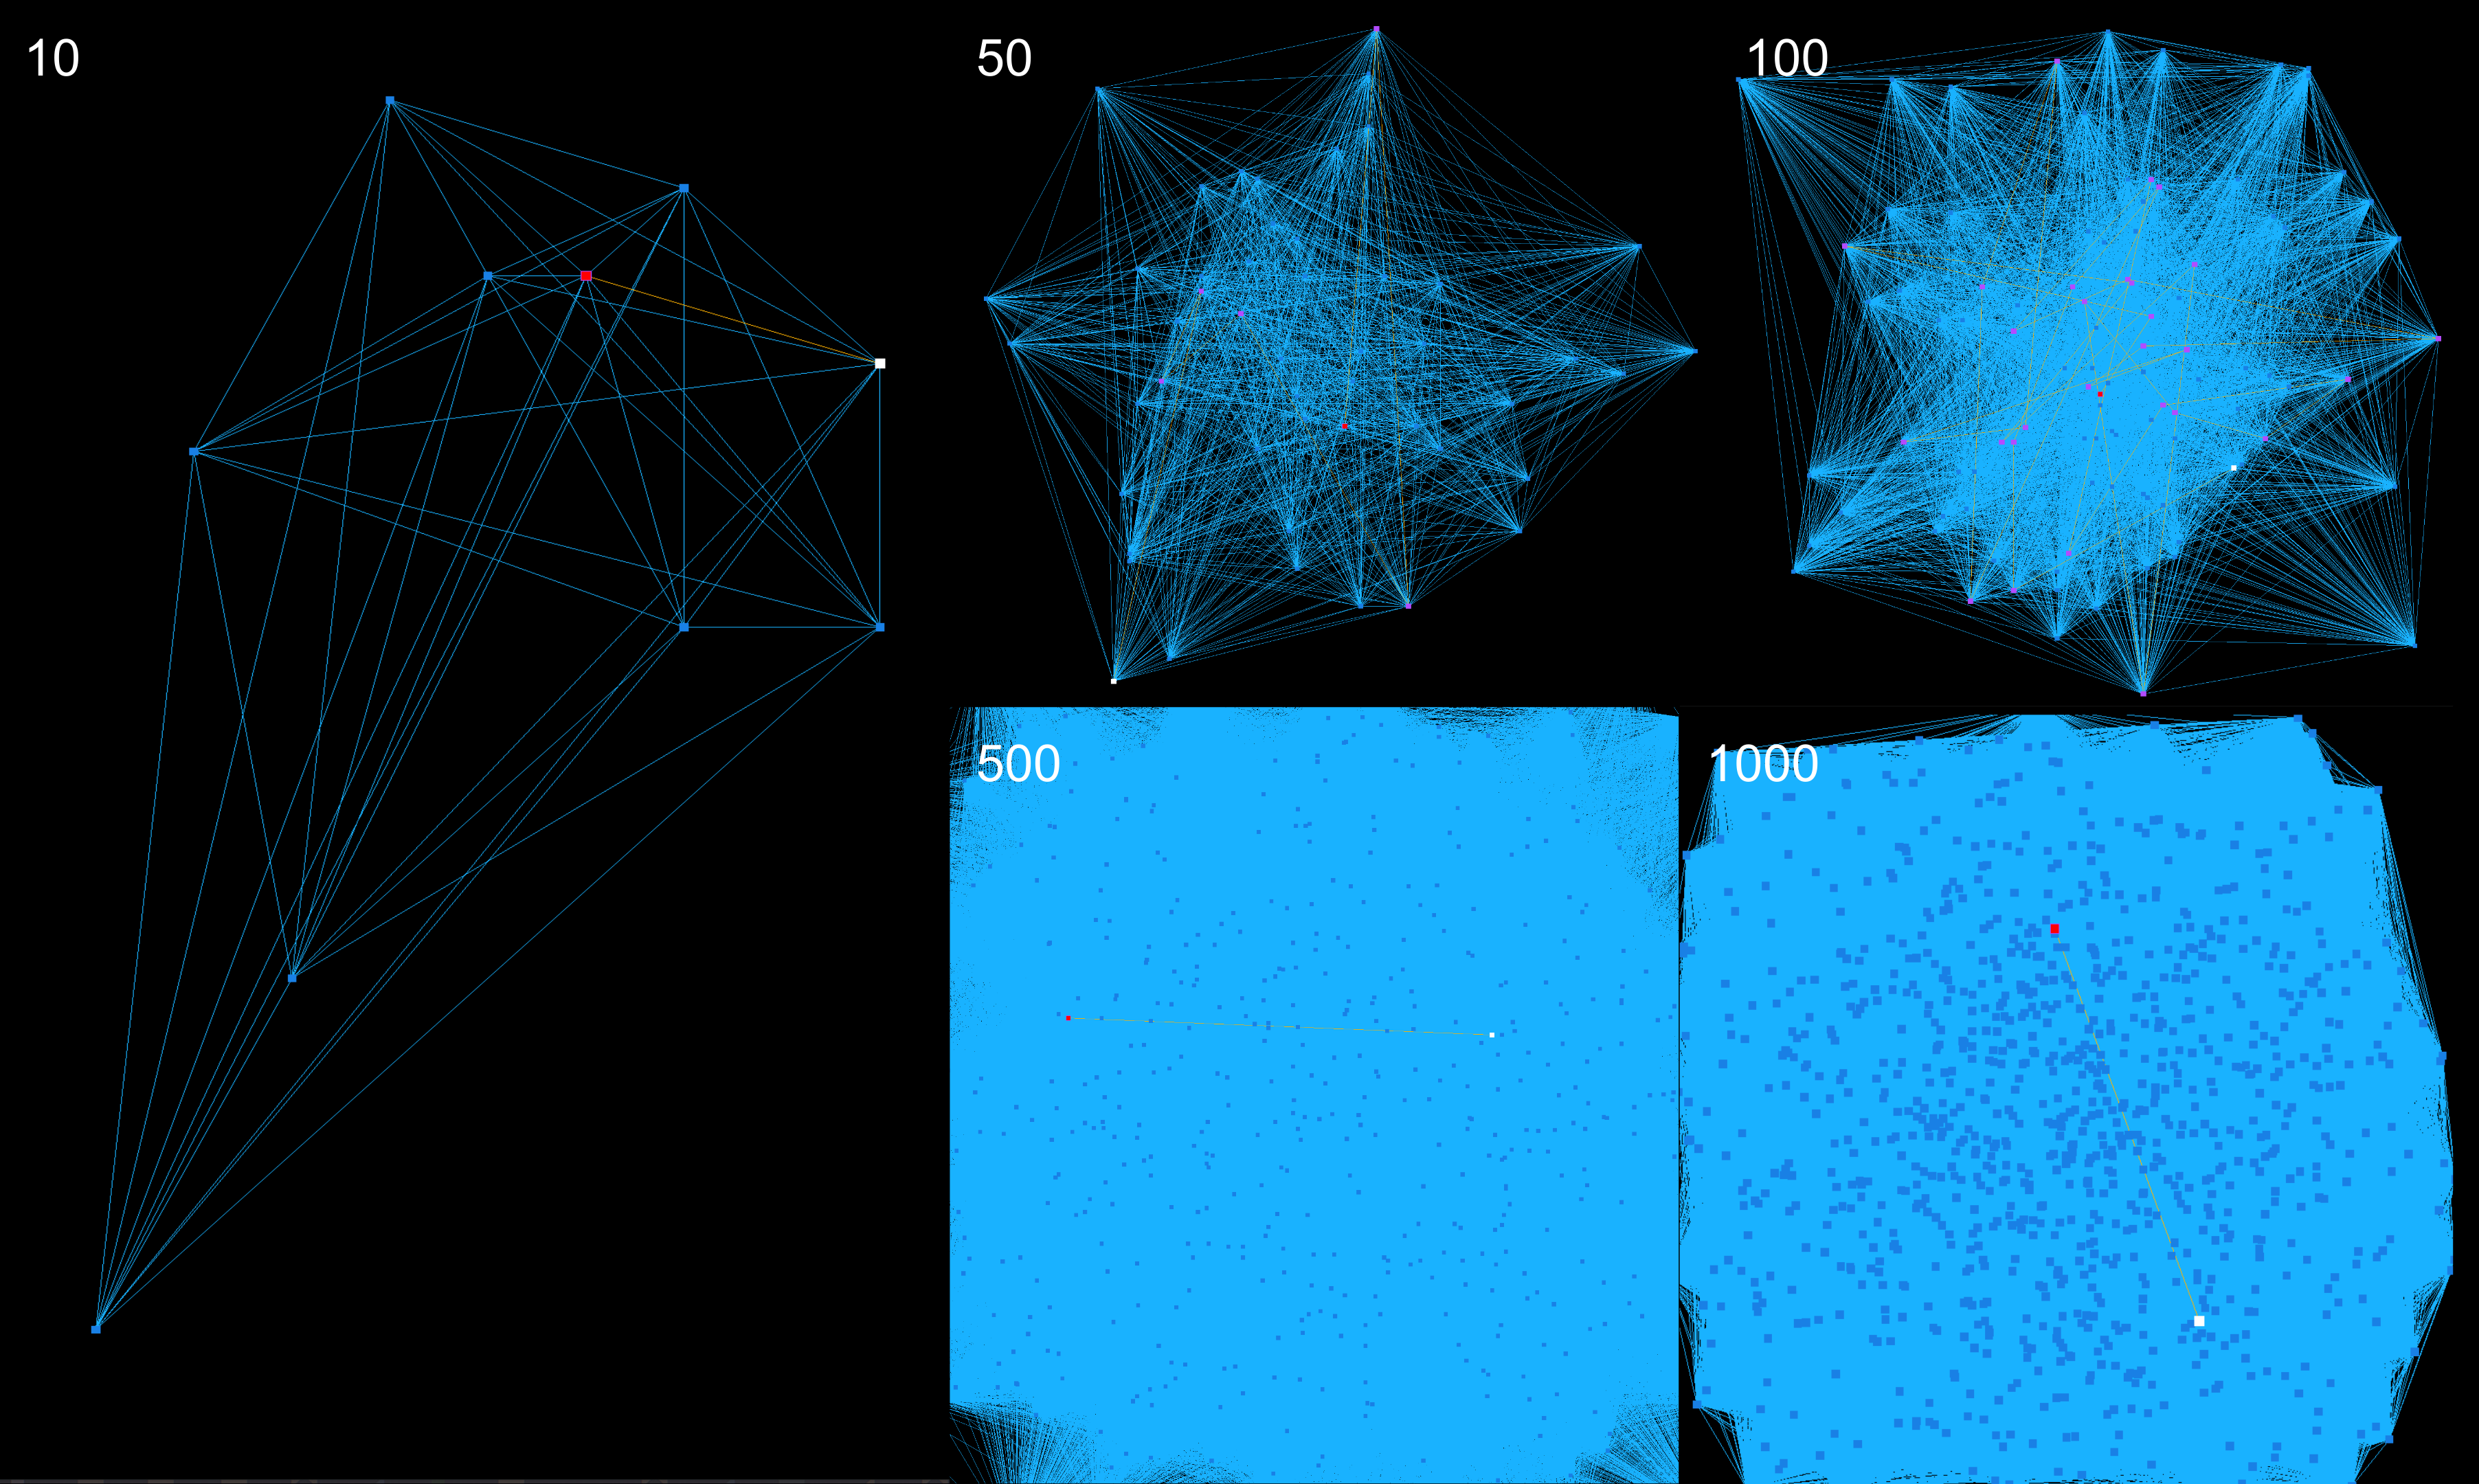
\includegraphics[width=0.7\textwidth]{Template_SBC/template-latex/grafoc.png}
\caption{This figure shows a compilation of the complete graphs obtained in the experiments. The number of nodes is indicated in the upper left corner of each one.}
\label{fig:exampleFig2}
\end{figure}

\begin{figure}[ht]
\centering
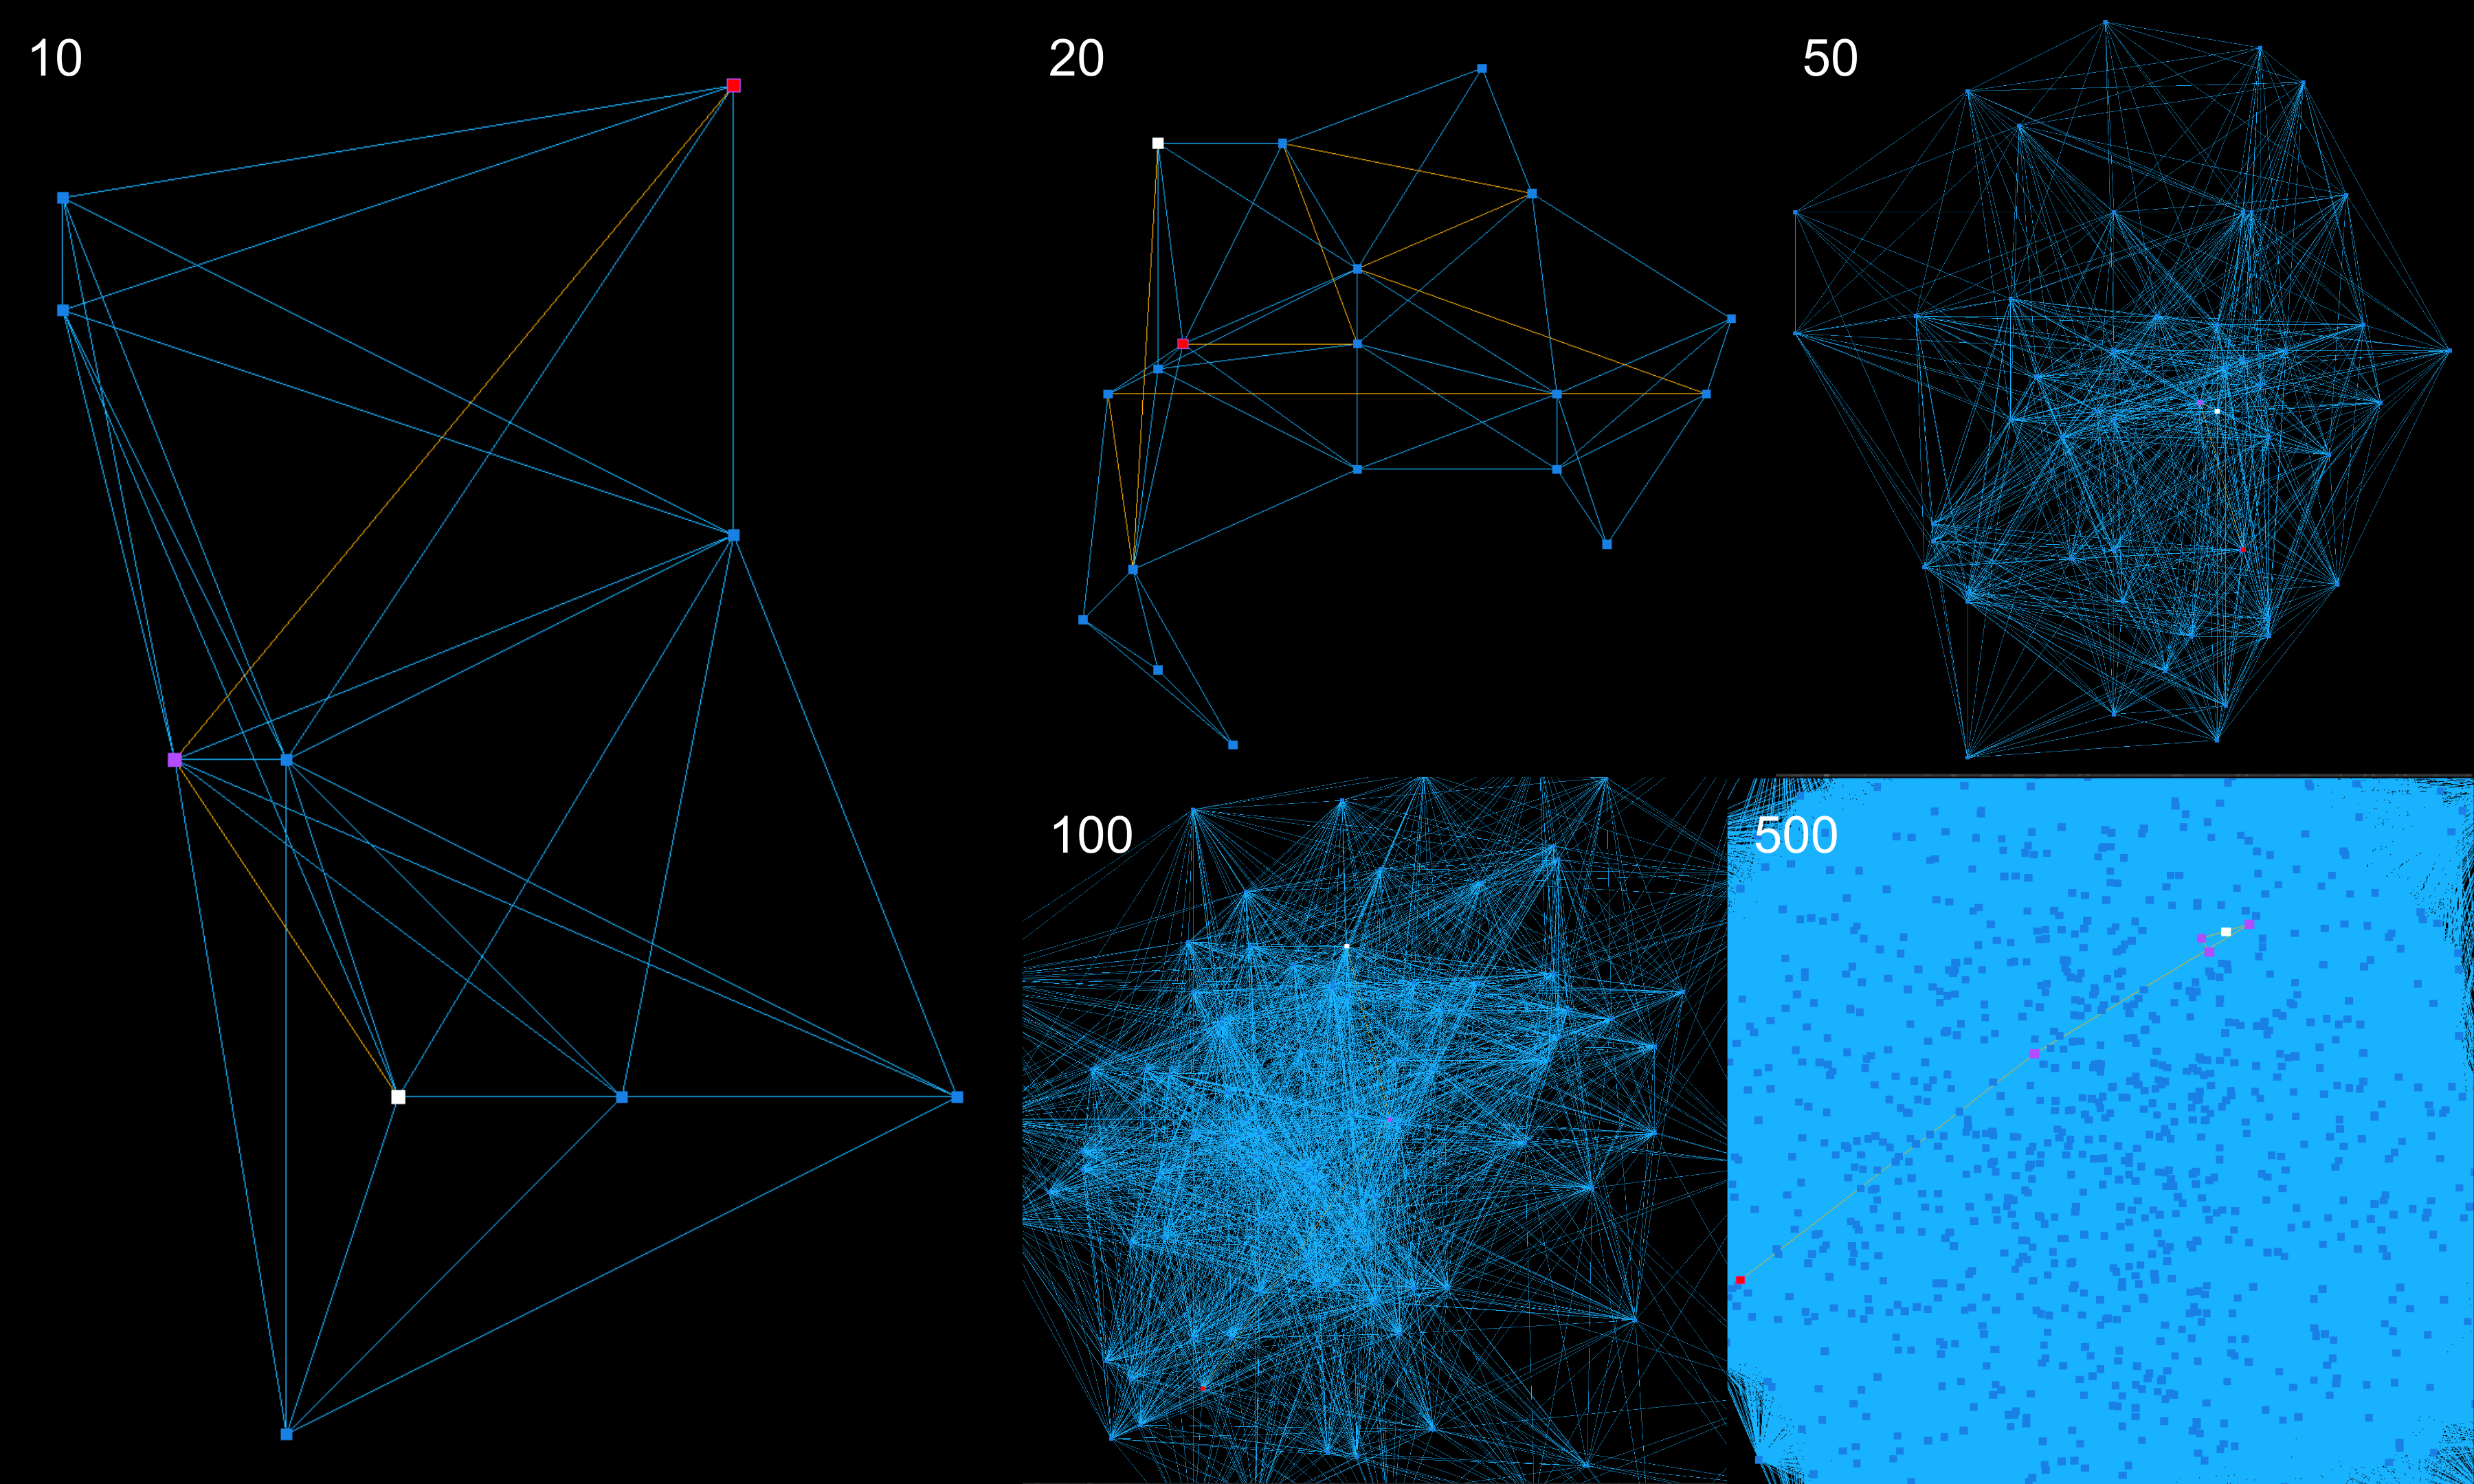
\includegraphics[width=0.7\textwidth]{Template_SBC/template-latex/grafonc.png}
\caption{This figure shows the incomplete graphs generated from different experiments and the number of nodes of each one.}
\label{fig:exampleFig3}
\end{figure}
\subsection{Results}
The table \ref{tab:my-table} shows the path size, execution time in milliseconds and cost of each of the experiments. The methods and their metrics are shown in each column and the experiments in each row.
The last row represents the average of the values in each column, for example the average run time for the 14 DFS experiments is 101,949 ms.

There are also boxes highlighted in gray that indicate the best value per row for each of the 3 parameters, in case of a tie both are highlighted.
In the case of 'Path size', the algorithm that achieves the objective in the fewest steps is considered the best, for 'E.Time (ms)' the one that performs the search in the shortest time is better and for 'Cost', the one that has a lower cost or distance.

The color of the text is also an indicator. The red color indicates that a path has not been found, this was generally given in heuristic methods since they try to find the most optimal path and discard various possible paths or have are based on a local search without backtracking.
The blue color highlights the best method for each experiment, based on the number of gray squares it has (better in some way), in case of a tie each metric is evaluated.
The green color represents represents the best by exception, for example in the case of having incomplete paths the second best or third is chosen, discarding the incomplete ones. Or in case the gray squares are not concentrated in a method, each metric is evaluated.

From the experiments we can deduce the following.
\begin{itemize}
    \item Method that has better characteristics
    \begin{enumerate}
    \item The hill climbing method was the best for 9 experiments, more than half.
    \item The best method is followed by A * with 4 experiments won.
    \item Finally, BFS has an experiment in which it is better, since the heuristic methods did not reach a path.
    \end{enumerate}
    \item{Completeness Problem: }Hill climbing failed twice and A * on 1 occasion
    \item{Winner according to the metric}
    \begin{enumerate}
        \item Path Size: Hill Climbing
        \item E.Time (ms): BFS
        \item Cost: A *
    \end{enumerate}
\end{itemize}



\begin{landscape}
\begin{longtable}[c]{|c|c|l|l|l|l|l|l|l|l|l|l|l|l|}
\hline
\multicolumn{2}{|c|}{} &
  \multicolumn{6}{c|}{\textbf{Blind}} &
  \multicolumn{6}{c|}{\textbf{Heuristic}} \\ \cline{3-14} 
\multicolumn{2}{|c|}{\multirow{-2}{*}{\textbf{Search}}} &
  \multicolumn{3}{c|}{\textbf{DFS}} &
  \multicolumn{3}{c|}{\textbf{BFS}} &
  \multicolumn{3}{c|}{\textbf{A*}} &
  \multicolumn{3}{c|}{\textbf{Hill Climbing}} \\ \hline
\endhead
%
\multicolumn{2}{|c|}{\textbf{Features}} &
  \multicolumn{1}{c|}{} &
  \multicolumn{1}{c|}{} &
  \multicolumn{1}{c|}{} &
  \multicolumn{1}{c|}{} &
  \multicolumn{1}{c|}{} &
  \multicolumn{1}{c|}{} &
  \multicolumn{1}{c|}{} &
  \multicolumn{1}{c|}{} &
  \multicolumn{1}{c|}{} &
  \multicolumn{1}{c|}{} &
  \multicolumn{1}{c|}{} &
  \multicolumn{1}{c|}{} \\ \cline{1-2}
\textbf{\#N} &
  \textbf{Comp.} &
  \multicolumn{1}{c|}{\multirow{-2}{*}{\textbf{\begin{tabular}[c]{@{}c@{}}Path\\ size\end{tabular}}}} &
  \multicolumn{1}{c|}{\multirow{-2}{*}{\textbf{\begin{tabular}[c]{@{}c@{}}E.Time\\ (ms)\end{tabular}}}} &
  \multicolumn{1}{c|}{\multirow{-2}{*}{\textbf{Cost}}} &
  \multicolumn{1}{c|}{\multirow{-2}{*}{\textbf{\begin{tabular}[c]{@{}c@{}}Path\\ size\end{tabular}}}} &
  \multicolumn{1}{c|}{\multirow{-2}{*}{\textbf{\begin{tabular}[c]{@{}c@{}}E.Time\\ (ms)\end{tabular}}}} &
  \multicolumn{1}{c|}{\multirow{-2}{*}{\textbf{Cost}}} &
  \multicolumn{1}{c|}{\multirow{-2}{*}{\textbf{\begin{tabular}[c]{@{}c@{}}Path\\ size\end{tabular}}}} &
  \multicolumn{1}{c|}{\multirow{-2}{*}{\textbf{\begin{tabular}[c]{@{}c@{}}E.Time\\ (ms)\end{tabular}}}} &
  \multicolumn{1}{c|}{\multirow{-2}{*}{\textbf{Cost}}} &
  \multicolumn{1}{c|}{\multirow{-2}{*}{\textbf{\begin{tabular}[c]{@{}c@{}}Path\\ size\end{tabular}}}} &
  \multicolumn{1}{c|}{\multirow{-2}{*}{\textbf{\begin{tabular}[c]{@{}c@{}}E.Time\\ (ms)\end{tabular}}}} &
  \multicolumn{1}{c|}{\multirow{-2}{*}{\textbf{Cost}}} \\ \hline
 &
  \textbf{Y} &
  3 &
  0.022 &
  15.1333 &
  9 &
  0.02 &
  67.2523 &
  \cellcolor[HTML]{C0C0C0}2 &
  0.023 &
  \cellcolor[HTML]{C0C0C0}2.23607 &
  \cellcolor[HTML]{C0C0C0}{\color[HTML]{00009B} 2} &
  \cellcolor[HTML]{C0C0C0}{\color[HTML]{00009B} 0.19} &
  \cellcolor[HTML]{C0C0C0}{\color[HTML]{00009B} 2.23607} \\ \cline{2-14} 
\multirow{-2}{*}{\textbf{10}} &
  \textbf{N} &
  10 &
  0.032 &
  24.1785 &
  5 &
  \cellcolor[HTML]{C0C0C0}0.012 &
  14.8072 &
  \cellcolor[HTML]{C0C0C0}2 &
  0.024 &
  \cellcolor[HTML]{C0C0C0}6.32456 &
  \cellcolor[HTML]{C0C0C0}{\color[HTML]{00009B} 2} &
  \cellcolor[HTML]{FFFFFF}{\color[HTML]{00009B} 0.018} &
  \cellcolor[HTML]{C0C0C0}{\color[HTML]{00009B} 6.32456} \\ \hline
 &
  \textbf{Y} &
  7 &
  \cellcolor[HTML]{C0C0C0}0.055 &
  254.153 &
  47 &
  0.061 &
  1645.44 &
  \cellcolor[HTML]{C0C0C0}2 &
  0.086 &
  \cellcolor[HTML]{C0C0C0}44.6878 &
  \cellcolor[HTML]{C0C0C0}{\color[HTML]{00009B} 2} &
  {\color[HTML]{00009B} 0.08} &
  \cellcolor[HTML]{C0C0C0}{\color[HTML]{00009B} 44.6878} \\ \cline{2-14} 
\multirow{-2}{*}{\textbf{50}} &
  \textbf{N} &
  13 &
  0.067 &
  166.22 &
  44 &
  \cellcolor[HTML]{C0C0C0}0.045 &
  715.09 &
  \cellcolor[HTML]{C0C0C0}3 &
  0.07 &
  \cellcolor[HTML]{C0C0C0}19.9561 &
  \cellcolor[HTML]{C0C0C0}{\color[HTML]{00009B} 3} &
  {\color[HTML]{00009B} 0.063} &
  \cellcolor[HTML]{C0C0C0}{\color[HTML]{00009B} 19.9561} \\ \hline
 &
  \textbf{Y} &
  60 &
  0.151 &
  4375.48 &
  30 &
  \cellcolor[HTML]{C0C0C0}0.01 &
  1759.3 &
  \cellcolor[HTML]{C0C0C0}2 &
  0.038 &
  \cellcolor[HTML]{C0C0C0}39.4462 &
  \cellcolor[HTML]{C0C0C0}{\color[HTML]{00009B} 2} &
  {\color[HTML]{00009B} 0.033} &
  \cellcolor[HTML]{C0C0C0}{\color[HTML]{00009B} 39.4462} \\ \cline{2-14} 
\multirow{-2}{*}{\textbf{100}} &
  \textbf{N} &
  46 &
  0.104 &
  1439.16 &
  23 &
  \cellcolor[HTML]{C0C0C0}0.008 &
  650.663 &
  {\color[HTML]{036400} 4} &
  {\color[HTML]{036400} 0.039} &
  \cellcolor[HTML]{C0C0C0}{\color[HTML]{036400} 101.829} &
  \cellcolor[HTML]{C0C0C0}3 &
  0.034 &
  109.776 \\ \hline
 &
  \textbf{Y} &
  42 &
  0.454 &
  14382.9 &
  21 &
  \cellcolor[HTML]{C0C0C0}0.007 &
  8103.29 &
  \cellcolor[HTML]{C0C0C0}2 &
  0.592 &
  \cellcolor[HTML]{C0C0C0}432.334 &
  \cellcolor[HTML]{C0C0C0}{\color[HTML]{00009B} 2} &
  {\color[HTML]{00009B} 0.192} &
  \cellcolor[HTML]{C0C0C0}{\color[HTML]{00009B} 432.334} \\ \cline{2-14} 
\multirow{-2}{*}{\textbf{500}} &
  \textbf{N} &
  155 &
  1.681 &
  22679.9 &
  423 &
  \cellcolor[HTML]{C0C0C0}0.095 &
  61618.9 &
  {\color[HTML]{036400} 4} &
  {\color[HTML]{036400} 0.643} &
  \cellcolor[HTML]{C0C0C0}{\color[HTML]{036400} 295.431} &
  \cellcolor[HTML]{C0C0C0}{\color[HTML]{9A0000} 3} &
  {\color[HTML]{9A0000} 0.239} &
  {\color[HTML]{9A0000} 305.566} \\ \hline
 &
  \textbf{Y} &
  479 &
  8.333 &
  369845 &
  761 &
  \cellcolor[HTML]{C0C0C0}0.14 &
  561553 &
  \cellcolor[HTML]{C0C0C0}2 &
  1.694 &
  \cellcolor[HTML]{C0C0C0}1009.37 &
  \cellcolor[HTML]{C0C0C0}{\color[HTML]{00009B} 2} &
  {\color[HTML]{00009B} 0.693} &
  \cellcolor[HTML]{C0C0C0}{\color[HTML]{00009B} 1009.37} \\ \cline{2-14} 
\multirow{-2}{*}{\textbf{1000}} &
  \textbf{N} &
  375 &
  6.943 &
  106020 &
  813 &
  \cellcolor[HTML]{C0C0C0}0.153 &
  224880 &
  6 &
  1.98 &
  \cellcolor[HTML]{C0C0C0}1264.81 &
  \cellcolor[HTML]{C0C0C0}{\color[HTML]{036400} 5} &
  {\color[HTML]{036400} 0.783} &
  {\color[HTML]{036400} 1476.18} \\ \hline
 &
  \textbf{Y} &
  1840 &
  153.077 &
  6.80316e+06 &
  920 &
  \cellcolor[HTML]{C0C0C0}0.161 &
  3.258e+06 &
  \cellcolor[HTML]{C0C0C0}{\color[HTML]{00009B} 2} &
  {\color[HTML]{00009B} 51.328} &
  \cellcolor[HTML]{C0C0C0}{\color[HTML]{00009B} 2743.08} &
  \cellcolor[HTML]{C0C0C0}2 &
  55.802 &
  \cellcolor[HTML]{C0C0C0}2743.08 \\ \cline{2-14} 
\multirow{-2}{*}{\textbf{5000}} &
  \textbf{N} &
  3242 &
  258.704 &
  4.88624e+06 &
  1621 &
  \cellcolor[HTML]{C0C0C0}0.3 &
  2.49728e+06 &
  \cellcolor[HTML]{C0C0C0}{\color[HTML]{00009B} 3} &
  {\color[HTML]{00009B} 52.477} &
  \cellcolor[HTML]{C0C0C0}{\color[HTML]{00009B} 4391} &
  \cellcolor[HTML]{C0C0C0}3 &
  54.227 &
  4408.22 \\ \hline
 &
  \textbf{Y} &
  4537 &
  738.471 &
  3.29035e+07 &
  7732 &
  \cellcolor[HTML]{C0C0C0}1.367 &
  5.66735e+07 &
  \cellcolor[HTML]{C0C0C0}2 &
  194.085 &
  \cellcolor[HTML]{C0C0C0}9182.16 &
  \cellcolor[HTML]{C0C0C0}{\color[HTML]{00009B} 2} &
  {\color[HTML]{00009B} 193.342} &
  \cellcolor[HTML]{C0C0C0}{\color[HTML]{00009B} 9182.16} \\ \cline{2-14} 
\multirow{-2}{*}{\textbf{10 000}} &
  \textbf{N} &
  1503 &
  259.197 &
  4.30721e+06 &
  {\color[HTML]{036400} 9249} &
  \cellcolor[HTML]{C0C0C0}{\color[HTML]{036400} 1.519} &
  {\color[HTML]{036400} 2.68546e+07} &
  {\color[HTML]{9A0000} 6} &
  {\color[HTML]{9A0000} 208.628} &
  \cellcolor[HTML]{C0C0C0}{\color[HTML]{9A0000} 7755.03} &
  \cellcolor[HTML]{C0C0C0}{\color[HTML]{9A0000} 4} &
  {\color[HTML]{9A0000} 220.049} &
  {\color[HTML]{9A0000} 9006.27} \\ \hline
\multicolumn{2}{|l|}{\textbf{Average}} &
  \textbf{879.428} &
  \textbf{101.949} &
  \textbf{3529950.866} &
  \textbf{1549.857} &
  \cellcolor[HTML]{9B9B9B}{\color[HTML]{333333} \textbf{0.278}} &
  \textbf{6438884.838} &
  \textbf{3} &
  \textbf{36.550} &
  \cellcolor[HTML]{9B9B9B}{\color[HTML]{333333} \textbf{1949.121}} &
  \cellcolor[HTML]{9B9B9B}{\color[HTML]{333333} \textbf{2.642}} &
  \textbf{37.553} &
  \textbf{2056.114} \\ \hline
\caption{Table of results when testing the 4 algorithms in 14 different experiments, in the last row the average of each column is shown.}
\label{tab:my-table}\\
\end{longtable}
\end{landscape}


\subsection{Comparison}
Following \cite{Maharshi2018ComparativeAO}, \cite{HLweb} and \cite{stuart2003artificial}, the performance of the algorithms can be compared based on the following parameters:
\begin{itemize}
    \item Time complexity: Time taken to find a solution.
    \item Space complexity: Memory required to perform the search.
    \item Optimality: Always find the minimum cost solution?
    \item Completeness: Always find the solution if it exists?
\end{itemize}
\begin{longtable}[c]{|c|c|c|c|c|}
\hline
\textbf{Algorithm}        & \textbf{DFS} & \textbf{BFS} & \textbf{A*} & \textbf{Hill Climbing} \\ \hline
\endhead
%
\textbf{Time Complexity}  & $O(b^{m})$   & $O(b^{d})$   & $O(b^{d})$  & $O(\infty)$            \\ \hline
\textbf{Space Complexity} & $O(bm)$      & $O(b^{d})$   & $O(b^{d})$  & $O(b)$             \\ \hline
\textbf{Optimality}       & No           & Yes          & Yes         & No                     \\ \hline
\textbf{Completeness}     & No           & Yes          & Yes         & No                     \\ \hline
\caption{Algorithm performance comparison}
\label{tab:my-table}
\end{longtable}
This theoretical comparison is reflected in the tested experiments, the bar chart \ref{tab:bc} shows the performance synthesis of each method. Proving that heuristic methods considerably reduce the cost and size of the road. But as it was seen previously they do not always arrive at the solution. An analysis by theoretical parameter was made.
\begin{itemize}
    \item Time complexity: the times obtained and the theoretical ones do not completely agree, but the best performance is A*.
    \item Space Complexity: This parameter was not considered in the experiments.
    \item Optimality: Theory and experiments agree that A * finds the least expensive solution and that DFS does not. But this does not match in BFS and hill climbing.
    \item Completeness: They coincide in BFS and Hill climbing that presents more problems.
\end{itemize}

\begin{figure}[ht]
\centering
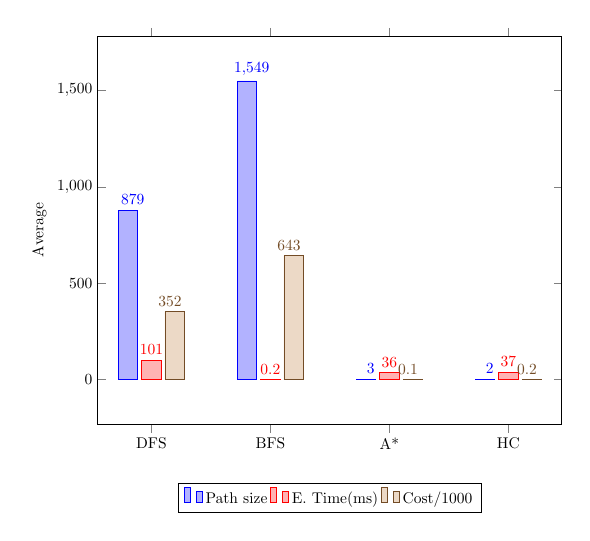
\begin{tikzpicture}[thick,scale=0.7, every node/.style={scale=0.8}]
\begin{axis}[
    ybar,
    enlargelimits=0.15,
    legend style={at={(0.5,-0.15)},
      anchor=north,legend columns=-1},
    ylabel={Average},
    symbolic x coords={DFS,BFS,A*,HC},
    xtick=data,
    nodes near coords,
    nodes near coords align={vertical},
    ]
\addplot coordinates {(DFS,879) (BFS,1549) (A*,3) (HC,2)};
\addplot coordinates {(DFS,101) (BFS,0.2) (A*,36) (HC,37)};
\addplot coordinates {(DFS,352) (BFS,643) (A*,0.1) (HC,0.2)};
\legend{Path size,E. Time(ms),Cost/1000}
\end{axis}
\label{tab:bc}
\end{tikzpicture}
\caption{Average of each metric for the 4 methods, the cost was divided into 1000 for practical purposes.}
\end{figure}
\section{Conclusions}
\begin{itemize}
    \item For the Shortest path problem, heuristic methods are better because they cost less.
    \item The search algorithms blind do not give the most optimal path but they are more secure.
    \item Incomplete graphs represent a greater challenge for heuristic methods.
    \item In the experiments it was found that the best performance is hill climbing but it can be disqualified for not being complete.
    \item A* has good performance and due to its optimality and completeness characteristics it can be considered the best option for the problem of finding paths between two points.
\end{itemize}

%\clearpage
\bibliographystyle{sbc}
\bibliography{sbc-template}
\clearpage

\begin{appendices}
  \section{Appendix: Main full code}
  \label{appendix:main}
  \lstinputlisting[language=C++, caption=Complete structure of the program, includes the graphic part. The codes of each method are in separate files.]{codes/main.cpp}
\end{appendices}

\includepdf{Template_SBC/contra-capa.pdf}
\end{document}
